\documentclass[journal, a4paper]{IEEEtran}

\usepackage{graphicx}   
\usepackage{url}        
\usepackage{amssymb}
\usepackage{amsmath}    
\usepackage{xcolor}
\newcommand\todo[1]{\textcolor{red}{#1}}

% Some useful/example abbreviations for writing math
\newcommand{\argmax}{\operatornamewithlimits{argmax}}
\newcommand{\argmin}{\operatornamewithlimits{argmin}}
\newcommand{\x}{\mathbf{x}}
\newcommand{\y}{\mathbf{y}}
\newcommand{\ypred}{\mathbf{\hat y}}
\newcommand{\yp}{{\hat y}}

\begin{document}

% Define document title, do NOT write author names for the initial submission
\title{Reinforcement Learning on 2048}
\author{Anonymous Authors}
\maketitle

% Write abstract here
\begin{abstract}
    In this project, we aim at training a game-playing agent for the 2048 game. 
    
    
% 	This document is a rough guide to producing the project report. You should enter the title, but do \emph{not} enter any author names or anything that identifies any of the authors (in any part of the document). 
% 	The structure (i.e., sections) outlined here is offered as as suggestion, but feel free to change if convenient. And, of course, replace these hints/instructions/examples with your own text. But you must use this IEEE template. 
	
% Hint: shared tools like \texttt{http://overleaf.com/} are great tools for collaborating on a multi-author report in \LaTeX. There are also Word templates (\url{https://www.ieee.org/conferences/publishing/templates.html}) if you wish; but you must convert to \texttt{pdf} format for submission. Recall the page limit of 5 pages.  
\end{abstract}

% Each section begins with a \section{title} command
\section{Introduction}
2048 is a game that went viral in 2014. The game's mathematical aspects and moderate complexity encouraged us to design a Reinforcement Learning agent that solves it\footnote{Code can be found using this link: \url{http://ourwetransferlink.zip}}. To achieve this, we implemented the game as an OpenAI Gym environment. In our implementation, the action space is discrete and features only four elements, but the state space grows exponentially with the board size. Since the number of states for a four by four game is bounded by $10^{18}$, it would be unfeasible to visit all the states to maximize the value function in each state, we opted for approximate algorithms such as Deep Q-Network (DQN). 

% \begin{enumerate}
% 	\item An overview of what you did, and why
% 	\item Provide access to your anonymous code.
% % 	Note that results should be reproducible using the technologies from the labs (i.e., Python, and relevant libraries)}. 
% \end{enumerate}


\section{Background and Related Work}

The best AI agent for 2048 we have found was developped by Robert Xiao \todo{[add reference 1]}. It implements an expectimax search in C++ and goes over 10,000,000 states per second. It has a $94\%$ chance of reaching the 16384 tile and $36\%$ of reaching the 32768 tile. It uses heuristics to make the reward function more representative of the strategy we would want an agent to follow. We further discuss these heuristics in section III.

In \todo{[add reference 2]}, the authors use N-tuple networks (NTNs) they achieve a highest score of 261526 which means that the agent was able to reach the 16384 tile. This agent is outperformed by \todo{[add reference 1]} and uses up to $2 \cdot 10^9$ parameters. We will not further investigate this method.

In \todo{[add reference 3]}, the authors use imitation learning to train their agent: A Convolutional Neural Network (CNN) is implemented with the grid state as input and a 4-dimention vector representing the probability for each action as output, the network is then updated based on the action chosen by an experimented player. Their agents performs worse than \todo{[add reference 2]}. Still, it reaches the 16384 tile $2\%$ of the time and the 4096 tile $57\%$ of the time.

% the authors compare different RL methods aimed at developing a game-playing agent for 2048. In particular, they test a method called N-Tuple Networks 

In \todo{[reference to MIT article]}, the authors implement a Probabilistic Policy Network which they try to improve using Approximate Dynamic Programming and Monte-Carlo Tree Search. However, their agent never reach the 2048 tile. The maximum tile it reaches is 1024.

As reinforcement becomes more and more widely used, more libraries that efficiently implement different RL methods emerge. Stable baseline \todo{[reference to stable baseline]} is a set of improved implementations of RL algorithms based on OpenAI Baselines that we use in order to create our agent.


% It is absolutely essential to provide sufficient background to your work. Elaborate (\emph{in your own words}) the material required to understand your work (for someone who has attended the course but needs a pedagogical reminder about the parts relevant to your project). 

% References are essential. You may cite lectures, e.g., \cite{Lecture3}, book chapters, e.g., Chapter x from \cite{Barber}, or articles from the literature, e.g., \cite{Astar,DeepMindSC2}, even blog posts and code repositories. In all cases you \emph{must} properly cite any work that is not your own.

% Don't hesitate to use and reference equations, but rigorously check that each part of your notation is introduced clearly. For example, Eq.~\eqref{eq:MAP} is a multi-label prediction, conditioned on input $\x \in \mathbb{R}^D$ (where $D$ is the input dimension), with regard to outputs $\y \in \{0,1\}^L$ for $L$ labels. 

% \begin{equation}
% 	\label{eq:MAP}
% 	% Note the example \newcommand s defined above which make it faster to write latex math
% 	\ypred = \argmax_{\y \in \{0,1\}^L} P(\y|\x)
% \end{equation}

\section{The Environment}

2048 is a fully-observed stochastic game played on a 4x4 grid. Every turn, the player chooses an action $a \in \textit{A}=\{ up, right, down, left \}$. Some cells of the grid contain tiles whose values are some power of 2. When the player chooses an action, all the tiles of the grid move along the chosen direction. If two tiles are adjacent and share the same value, they are merged into one single tile. The value of the new tile is the sum of values of the merged tiles. Each newly generated tile cannot merge with another tile in the same turn. After every turn, if the chosen action is valid (i.e. changes the configuration of the grid), a new tile of value 2 or 4 appears randomly in one of the remaining cells. 

The game ends if none of the remaining actions are valid. The goal of the player is to maximize his score (i.e. reward function). Initially the score is set to $0$ and the grid contains only one tile of value 2 or 4. After every merge operation, the score is incremented by the value of the newly generated tile. 

Some versions of this game consider the player a winner if he reaches the 2048 tile. We do not implement this version, the game goes on even if the 2048 tile is reached.

The goal of this project is to test different reinforcement learning algorithms in order to train an agent that performs well on this game. An experienced human should be able to reach the 2048 quite often.
% \todo{ Try to look for some statistics, I didn't find any at the moment. } 

One of the main challenges of this game is the exponential number of board configurations (i.e. states) which is bounded by $10^{18}$, which makes it impossible to use standard techniques that require visiting all the states.
% \todo{ Add screenshots of the console game.}

\begin{figure}[ht]
	\centering
	\begin{subfigure}
        \centering
        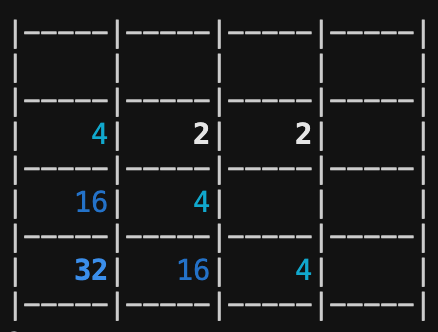
\includegraphics[width=.4\linewidth]{report/images/2048_board_1.png}
        % \caption{A subfigure}
        \label{fig:sub1}
    \end{subfigure}%
    \begin{subfigure}
      \centering
      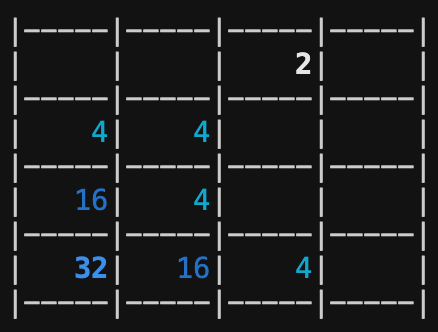
\includegraphics[width=.4\linewidth]{report/images/2048_board_2.png}
    %   \caption{A subfigure}
      \label{fig:sub2}
    \end{subfigure}
    \caption{On the left is a random grid configuration and on the right is the new configuration after the action $left$ has been chosen. Note that the two 2-tiles have merged into a 4-tile and a new 2-tile has appeared.}
% 	\caption{\label{env_figure}Figure captions should be descriptive (not like this one). }
\end{figure}

\subsection*{Representing the states} 
There are two possible ways to represent the states:
\begin{enumerate}
    \item an array of size 16 where each cell contains 0 if it's empty or the log of the tile it contains otherwise. The value of the log can never exceed 18 on a 4x4 grid. We can even suppose that it's bounded by 15 if we settle for the 32768 tile.
    \item we can represent each cell $i$ by a vector $u_i \in \{0,1\}^{16}$ where $u_i(j) = 1$ if, and only if, the cell $i$ contains the $2^j$-tile (or is empty if $j = 0$). A grid configuration is then represented as a $\{0,1\}^{256}$ vector.
\end{enumerate}
The second option is more widely used and has the advantage of making the cell values equidistant. Depending on what algorithm we use one representation or the other.

\subsection*{Improving the reward function using heuristics}
The score a normal player would want to maximize is the sum of values of all the generated tiles as stated earlier.
The reward at a given time step is the difference between the new state value and the previous state value.
However, in order to make it easier for our agent to better perform on this task, we tested a few heuristics inspired by \todo{[reference of the article]}. 

The new reward function is a weighted sum of four terms:
\begin{itemize}
    \item \textbf{Empty}: this term is equal to the number of empty of tiles on the board. The only parameter of this term is the weight;
    \item \textbf{Merges:} this term is equal to the number of possible merges on the board. The only parameter of this term is the weight;
    \item \textbf{Monotonicty:}: this term rewards rows or columns for having a (eventually partial) monotonic order. Each time it finds a correctly ordered neighbouring tiles, a reward of $B^x - S^x$ is given, with $B$, $S$ and $x$ being the bigger logarithm, the smaller logarithm and the monotonicity exponent parameter, respectively. The maximum of both directions for each line is its value and the board's values is the sum over all rows and columns. It has two parameters: the weight and the exponent.
    \item \textbf{Sum:} this term is the sum of the logarithm of all tiles elevated to a constant power, which is a parameter. It has two parameters: the weight and the exponent.
    
We also add a negative penalty if the agents chooses an invalid action.

    

\end{itemize}


% Describe your environment, addressing the following points:

% \begin{itemize}
% 	\item State space; What observations does an agent have of the environment
% 	\item Action space: what actions can be taken in this environment
% 	\item How is the reward function defined
% 	\item Is the environment deterministic or stochastic, fully observed, partially observed, not observed, etc. 
% 	\item What are the main challenges this environment poses (for an agent)
% 	\item Are there potential real-world applications, or is it for theoretical/educational interest?
% \end{itemize}

% Don't hesitate to use diagrams, figures, and screenshots wherever they are useful; as exemplified in Fig.~\ref{env_figure}.  


\section{The Agent}

As we mentioned before, the large state space makes the usage of tabular methods unfeasible due to computational limitations. Instead, we opted to concentrate our efforts on approximate algorithms. Despite, most of the Deep Learning methods we found in the literature estimate the policy directly - many by imitation learning from a human agent - we chose to focus on state-action value estimation techniques. Our objective is to test our hypothesis that DQN-based agents may be able to achieve good performance without the help of imitation learning. We experiment with both Multi-Layer Perceptron (MLP) and CNN policies. We expect CNN's to achieve better performance because they can take advantage of the board organization and learn local features.


% Describe your agent, answering the following points:
% \begin{itemize}
% 	\item What type(s) of agent(s) did you select/design for this environment, 
% 	\item Why this selection/design?
% 	\item What are the main advantages/disadvantages.
% 	\item How did you implement/configure/parametrize it. 
% \end{itemize}

\section{Results and Discussion}
This section is to be developed for the final submission.

% This is one of the most important sections. 
% \begin{enumerate}
% 	\item Test your agent(s) in the environment(s), 
% 	\item show the results, -- and most importantly -- 
% 	\item discuss and \emph{interpret} the results (don't just explain the results, but say what they mean); this includes highlighting strong points and also weaknesses.
% \end{enumerate}

% Make use of plots, e.g., Fig.~\ref{results_figure}, tables (e.g., Table~\ref{results_table}), etc; anything that illustrates the performance of your agent in the environment under different configurations. Make sure to clearly indicate which parameters ($\gamma$, etc.) you have set. 

% \begin{figure}[ht]
% 	\centering
% 	\includegraphics[width=0.8\columnwidth]{results_plot.pdf}
% 	\caption{\label{results_figure}An example plot. Your plots should be understandable from labels and the caption.}
% \end{figure}

\begin{table}[ht]
	\caption{\label{results_table}Table captions should adequately describe the contents of tables (unlike this one).}
	\centering
	\begin{tabular}{lll}
		\hline
		\textbf{Environment config.} & \textbf{SARSA} & \textbf{Q-Learning}  \\
		\hline
		Simulation 1        & 10             & 15 \\
		Simulation 2        & 12             & 11 \\
		\hline
	\end{tabular}
\end{table}

\section{Conclusion and Future Work}
	Summarize the project: Main outcome, discoveries, lessons learned, possible future work if you had had more time, etc. %Also remark about what would be the next steps you would take if you or someone else were to continue/extend this project. 

% The bibliography:
\begin{thebibliography}{4}

	\bibitem{2048-ai} % Book
	R. Xiao. https://github.com/nneonneo/2048-ai
% 	{\em Cambridge University Press}, 2012.

	\bibitem{Lecture3} % Web document
		As mentioned in Lecture III - Multi-Output Learning. \textit{INF581 Advanced Topics in Artificial Intelligence}, 2020.

	\bibitem{Astar}
	D.~Mena et al. A family of admissible heuristics for A* to perform inference in probabilistic classifier chains.
	{\em Machine Learning}, vol. 106, no. 1, pp 143-169, 2017.

	\bibitem{DeepMindSC2}
	O.~Vinyals et al. StarCraft {II:} {A} New Challenge for Reinforcement Learning.
	\url{https://arxiv.org/abs/1708.04782}, 2017. 

\end{thebibliography}

\newpage
\section*{Appendix}
Some other interesting things you tried that aren't essential to the main outcome? (For example, additional results and tables, lengthy derivations, \ldots). You can include them here (does not count towards page limit). 
\end{document}
